\documentclass[a4paper, 11pt]{article}
\usepackage[T1]{fontenc}
\usepackage[utf8]{inputenc}
\usepackage[norsk]{babel}
\usepackage{graphicx}
\usepackage[dvipsnames]{xcolor}
\usepackage[fleqn]{amsmath}
\usepackage{amsthm, amssymb}
\usepackage{microtype}
\usepackage{array}
\usepackage{caption}
\usepackage{subcaption}
\usepackage[norsk]{babel}
\usepackage[all]{nowidow}
%\usepackage{indentfirst}
\usepackage{mathtools}
\usepackage{sectsty}
\usepackage{tikz}
\usetikzlibrary{calc,arrows,patterns}
\usepackage{pdfpages}
\usepackage{amssymb}
\usepackage{cancel}

% Unicode-inkompatibilitet mactex/texlive?
\DeclareUnicodeCharacter{00A0}{ }

% Få fancyhdr til å holde kjeft
\setlength{\headheight}{14pt} 

%-------------------------------------%
% Dokument-settings
%-------------------------------------%
\newcommand{\tittel}{Øving 2}
\newcommand{\fag}{Diskret Matematikk}
\newcommand{\fagkode}{TMA4140}
\newcommand{\forfatter}{Steffen Haug}


\renewcommand{\qedsymbol}{$\themecolor{\blacksquare}$}
\newcommand{\lheq}{\stackrel{\text{\tiny{L'Hop}}}{=}}
\newcommand{\ceq}[2]{\stackrel{\text{\tiny{#1}}}{#2}}
\newcommand{\R}{\mathbb{R}}
\newcommand{\vect}[1]{\mathbf{#1}}
\newcommand{\deloppg}[1]{\vspace{1mm}\noindent \textbf{\themecolor{#1:}}}
\newcommand{\steg}[1]{\vspace{1mm}\noindent {\themecolor{#1:}}}
\newcommand{\dint}{\int\displaylimits}

\newcommand{\cvec}[1]{\begin{bmatrix}#1\end{bmatrix}}

\newcommand{\themeshade}{Mahogany}
\newcommand{\themecolor}[1]{\textcolor{\themeshade}{#1}}
\sectionfont{\color{\themeshade}}

\DeclarePairedDelimiter\abs{\lvert}{\rvert}
\def\dul#1{\underline{\underline{#1}}}
\def\multipart#1{
\left\{
	\begin{array}{ll}
		#1
	\end{array}
\right.
}


\usepackage{fancyhdr}
\lhead{\tittel \:{\color{\themeshade}\fagkode}}
\rhead{\forfatter}

\author{\forfatter}
\date{}

\newcommand*{\titleTH}{\begingroup % Create the command for including the title page in the document
\raggedleft % Right-align all text
\vspace*{\baselineskip} % Whitespace at the top of the page

{\Large \forfatter}\\[0.167\textheight] % Author name

{\LARGE\bfseries \tittel}\\[\baselineskip] % First part of the title, if it is unimportant consider making the font size smaller to accentuate the main title

{\themecolor{\Huge \fag}}\\[\baselineskip] % Main title which draws the focus of the reader

{\Large \textit{\fagkode}}\par % Tagline or further description

\vfill % Whitespace between the title block and the publisher
\endgroup}


\begin{document}

\pagestyle{empty}
\titleTH\newpage

\section{Oppgåver til seksjon 2.1} % 5 24
\subsection*{Oppgåve 5}

\deloppg{a} \( \{ 1,3,3,5,5,5,5,5 \} = \{5,3,1\}\)

\deloppg{b} \( \{\{1\}\} \neq \{1, \{1\}\} \)

\deloppg{c} \( \varnothing \neq \{\varnothing\} \)

\subsection*{Oppgåve 24}
\deloppg{a} \( \varnothing \) er ikkje potensmengde til nokon mengd.

\deloppg{b} \( \{\varnothing, \{a\} \} \) er potensmengde til \( \{a\} \)

\deloppg{c} \( \{ \varnothing, \{a\}, \{\varnothing, a\} \} 
= \{\varnothing,\{a\}\} \) er potensmengde til \(\{a\}\)

\deloppg{d} \( \{\varnothing, \{a\}, \{b\}, \{a,b\}\} \) er potensmengde til \(\{a,b\}\)


\section{Oppgåver til seksjon 2.2}

\subsection{Oppgåve 18}
\noindent La \(A,B,C\) vera mengder. Skal vise at

\deloppg{c} \( (A \setminus B) \setminus C \subseteq A \setminus C \)

\noindent Er det same som:
\begin{align*}
    &\{x \in A : x \not\in B, x \not\in C\} \subseteq \{x \in A : x \not\in C\} \\
    \intertext{Brukar definisjonen av delmengder:}
    &\forall x (x \in A \land x\not\in B \land x\not\in C) \rightarrow (x \in A \land x \not\in C))\\
    &\forall x (x \in (A\setminus B)\setminus C \rightarrow x \in A \setminus C) \\
    \implies &(A \setminus B)\setminus C \subseteq A \setminus C
\end{align*}

\deloppg{d} \( (A - C) \cap (C - B) = \varnothing\)

\noindent Er det same som:
\begin{align*}
    &\{x \in A : x \not\in C\} \cap \{x \in C : x \not\in B\} \\
    =&\{x: x \in A \land \themecolor{x \not\in C \land x \in C} \land x \not\in B \}
       \quad \themecolor{*}\; \text{\themecolor{motseiing}}\implies\text{predikatet alltid usant}\\
    \ceq{\themecolor{\(*\)}}{=}& \varnothing
\end{align*}


\newpage
\subsection*{Oppgåve 42} % stemmer, venn-diagram
Skal sjekke om gitt mengder \(A,B,C,D\), stemmer det at
\[
    (A \oplus B) \oplus (C \oplus D) = (A \oplus C) \oplus (B \oplus D)
\]

\begin{figure}[h]
    \begin{subfigure}{.25\textwidth}
        \centering
        \caption*{\themecolor{\(A \oplus B\)}}
        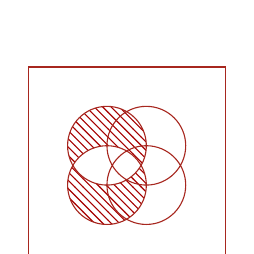
\begin{tikzpicture}[scale=.5]
            \begin{scope}[even odd rule]
                \clip (0,1) circle (1)
                      (0,0) circle (1);
                \fill [pattern color = Mahogany, pattern = north west lines] (0,1) circle (1);
                \fill [pattern color = Mahogany, pattern = north west lines] (0,0) circle (1);
            \end{scope}
            % outline
            \draw [Mahogany] (0,0) circle (1)  % B
                             (1,0) circle (1)  % D
                             (0,1) circle (1)  % A
                             (1,1) circle (1); % C
            \draw [Mahogany] (-2,-2) rectangle (3,3);
        \end{tikzpicture}
    \end{subfigure}
    \begin{subfigure}{.25\textwidth}
        \centering
        \caption*{\themecolor{\(C \oplus D\)}}
        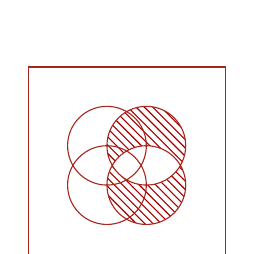
\begin{tikzpicture}[scale=.5]
            \begin{scope}[even odd rule]
                \clip (1,1) circle (1)
                      (1,0) circle (1);
                \fill [pattern color = Mahogany, pattern = north west lines] (1,1) circle (1);
                \fill [pattern color = Mahogany, pattern = north west lines] (1,0) circle (1);
            \end{scope}
            \draw [Mahogany] (0,0) circle (1)
                             (1,0) circle (1)
                             (0,1) circle (1)
                             (1,1) circle (1);
            \draw [Mahogany] (-2,-2) rectangle (3,3);
        \end{tikzpicture}
    \end{subfigure}
    \begin{subfigure}{.5\textwidth}
        \centering
        \caption*{\themecolor{\((A \oplus B) \oplus (C \oplus D)\)}}
        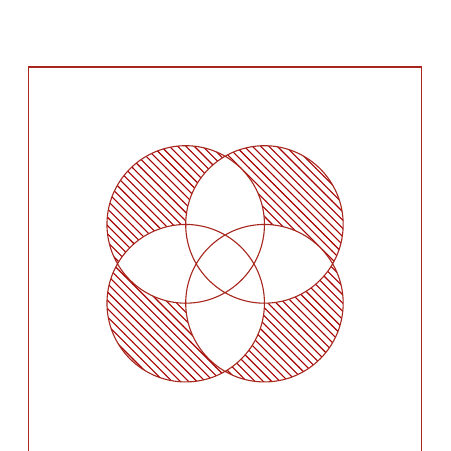
\begin{tikzpicture}
            \begin{scope}
                \fill [pattern color = Mahogany, pattern = north west lines] (0,1) circle (1);
                \clip (0,1) circle (1);
                \fill [white] (0,0) circle (1);
                \fill [white] (1,0) circle (1);
                \fill [white] (1,1) circle (1);
            \end{scope}
            \begin{scope}
                \fill [pattern color = Mahogany, pattern = north west lines] (0,0) circle (1);
                \clip (0,0) circle (1);
                \fill [white] (0,1) circle (1);
                \fill [white] (1,0) circle (1);
                \fill [white] (1,1) circle (1);
            \end{scope}
            \begin{scope}
                \fill [pattern color = Mahogany, pattern = north west lines] (1,0) circle (1);
                \clip (1,0) circle (1);
                \fill [white] (0,0) circle (1);
                \fill [white] (0,1) circle (1);
                \fill [white] (1,1) circle (1);
            \end{scope}
            \begin{scope}
                \fill [pattern color = Mahogany, pattern = north west lines] (1,1) circle (1);
                \clip (1,1) circle (1);
                \fill [white] (0,0) circle (1);
                \fill [white] (1,0) circle (1);
                \fill [white] (0,1) circle (1);
            \end{scope}
        % outline
            \draw [Mahogany] (0,0) circle (1)
                             (1,0) circle (1)
                             (0,1) circle (1)
                             (1,1) circle (1);
            \draw [Mahogany] (-2,-2) rectangle (3,3);
        \end{tikzpicture}
    \end{subfigure}
\end{figure}

\begin{figure}[h]
    \begin{subfigure}{.25\textwidth}
        \centering
        \caption*{\themecolor{\(A \oplus B\)}}
        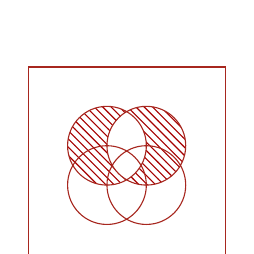
\begin{tikzpicture}[scale=.5]
            \begin{scope}[even odd rule]
                \clip (0,1) circle (1)
                      (1,1) circle (1);
                \fill [pattern color = Mahogany, pattern = north west lines] (0,1) circle (1);
                \fill [pattern color = Mahogany, pattern = north west lines] (1,1) circle (1);
            \end{scope}
            % outline
            \draw [Mahogany] (0,0) circle (1)  % B
                             (1,0) circle (1)  % D
                             (0,1) circle (1)  % A
                             (1,1) circle (1); % C
            \draw [Mahogany] (-2,-2) rectangle (3,3);
        \end{tikzpicture}
    \end{subfigure}
    \begin{subfigure}{.25\textwidth}
        \centering
        \caption*{\themecolor{\(C \oplus D\)}}
        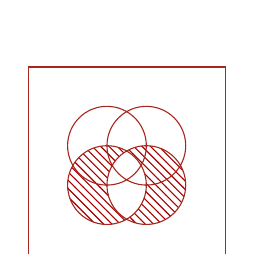
\begin{tikzpicture}[scale=.5]
            \begin{scope}[even odd rule]
                \clip (0,0) circle (1)
                      (1,0) circle (1);
                \fill [pattern color = Mahogany, pattern = north west lines] (0,0) circle (1);
                \fill [pattern color = Mahogany, pattern = north west lines] (1,0) circle (1);
            \end{scope}
            \draw [Mahogany] (0,0) circle (1)
                             (1,0) circle (1)
                             (0,1) circle (1)
                             (1,1) circle (1);
            \draw [Mahogany] (-2,-2) rectangle (3,3);
        \end{tikzpicture}
    \end{subfigure}
    \begin{subfigure}{.5\textwidth}
        \centering
        \caption*{\themecolor{\((A \oplus C) \oplus (B \oplus D)\)}}
        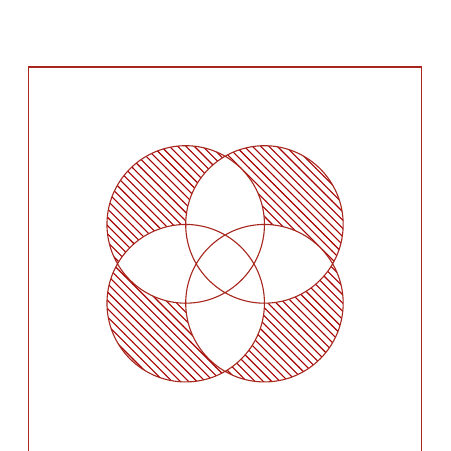
\begin{tikzpicture}
            \begin{scope}
                \fill [pattern color = Mahogany, pattern = north west lines] (0,1) circle (1);
                \clip (0,1) circle (1);
                \fill [white] (0,0) circle (1);
                \fill [white] (1,0) circle (1);
                \fill [white] (1,1) circle (1);
            \end{scope}
            \begin{scope}
                \fill [pattern color = Mahogany, pattern = north west lines] (0,0) circle (1);
                \clip (0,0) circle (1);
                \fill [white] (0,1) circle (1);
                \fill [white] (1,0) circle (1);
                \fill [white] (1,1) circle (1);
            \end{scope}
            \begin{scope}
                \fill [pattern color = Mahogany, pattern = north west lines] (1,0) circle (1);
                \clip (1,0) circle (1);
                \fill [white] (0,0) circle (1);
                \fill [white] (0,1) circle (1);
                \fill [white] (1,1) circle (1);
            \end{scope}
            \begin{scope}
                \fill [pattern color = Mahogany, pattern = north west lines] (1,1) circle (1);
                \clip (1,1) circle (1);
                \fill [white] (0,0) circle (1);
                \fill [white] (1,0) circle (1);
                \fill [white] (0,1) circle (1);
            \end{scope}
        % outline
            \draw [Mahogany] (0,0) circle (1)
                             (1,0) circle (1)
                             (0,1) circle (1)
                             (1,1) circle (1);
            \draw [Mahogany] (-2,-2) rectangle (3,3);
        \end{tikzpicture}
    \end{subfigure}
\end{figure}

\noindent Mengdene er like.


\section{Oppgåver til seksjon 2.3} % 12 38 42

\subsection*{Oppgåve 12}
Skal avgjere om funksjonane er ``ein til ein''

\deloppg{a} \(f(n) = n - 1\)
\begin{align*}
    \intertext{Sjekkar om \(f(a) = f(b) \implies a = b\)}
    a - 1 &= b - 1 \\
    a &= b \implies \text{funksjonen er 1-1}
\end{align*}

\deloppg{b} \(f(n) = n^2 + 1\)
\begin{align*}
    a^2 + 1 &= b^2 + 1 \\
    a^2 &= b^2 \\
    a &= \pm b \implies \text{funksjonen er ikkje 1-1}
\end{align*}

\deloppg{c} \(f(n) = n^3\)
\begin{align*}
    a^3 &= b^3 \\
    a &= b \implies \text{funksjonen er 1-1}
\end{align*}

\deloppg{d} \(f(n) = \left\lceil \frac{n}{2} \right\rceil \)

\vspace{3mm}
\noindent Moteksempel: \(f(1) = f(2) = 1 \implies \) funksjonen er ikkje 1-1


\subsection*{Oppgåve 38}
Skal finne begrensingar for \(a,b,c,d\) slik at \(f \circ g = g \circ f\). Altso
\begin{align*}
    f \circ g &= g \circ f \\
    a(cx + d) + b &= c(ax+b) + d \\
    acx + ad + b &= acx + bc + d \\
    ad + b &= bc + d \\
    d(a-1) &= b(c-1) \\
    \intertext{Som er oppfyld når:}
    a,c = 1 \\
    \intertext{eller}
    b,d = 0 \\
    \intertext{eller}
    a=c \\ b=d
\end{align*}

\newpage
\subsection*{Oppgåve 42}
Gitt \(f: \mathbb{R \rightarrow \mathbb{R}}, \quad f(x)=x^2\). Skal i prinsippet finne
definisjonsmengdene (til \(f\)) som gjev dei oppgjevne verdimengdene.

\vspace{3mm}
\deloppg{a} \(f^{-1}(\{1\})\) = \{1\}

\vspace{3mm}
\deloppg{b} \(f^{-1}(\{x : 0 < x < 1\}) = \{x : 0 < x < 1\}\)

\vspace{3mm}
\deloppg{c} \(f^{-1}(\{x: x > 4\}) = \{x : x > 2\}\)

\section{Oppgåver til seksjon 2.4} % 12c 33d

\subsection*{Oppgåve 12c}
Skal undersøkje om \(a_n = (-4)^n\) er løysing til \(a_n = 8a_{n-1} - 16a_{n-2}\)

\noindent \(\forall n > 2\):
\begin{align*}
    (-4)^n &= 8(-4)^{n-1} - 16(-4)^{n-2} \\
    &= -2(-4)(-4)^{n-1} - (-4)^2(-4)^{n-2} \\
    &= -2(-4)^n - (-4)^n \\
    \implies (-4)^n &= -3(-4)^n \quad \text{\themecolor{motseiing}}
\end{align*}

\noindent \(a_n = (-4)^n\) er {\em ikkje} løysing.


\subsection*{Oppgåve 33d}
Skal rekne ut summen
\begin{align*}
    &\sum_{i=1}^2\sum_{j=1}^3 ij \\
    =\;&\sum_{i=1}^2i\sum_{j=1}^3j \\
    =\;&3 \cdot 9 = \dul{21}\\
\end{align*}

\newpage
\section{Oppgåver til seksjon 2.5} % 16
\subsection*{Oppgåve 16}
Skal vise at ei delmengd av ei telleleg mengd (kall den \(S\)) sjølv er telleleg.

\begin{proof}
    At \(S\) er telleleg betyr at der eksisterar ein funksjon \(f: S \rightarrow \mathbb{N}\), slik at \(f\)
    er injiktiv for alle verdiar i \(S\).

    For ei kvar delmengd av \(S\), kall den \(S'\) kan ein definere ein 
    funksjon \(f|_{S'}: S' \rightarrow \mathbb{N}\). Sidan \(f|_{S'}\) berre er ei begrensing av \(f\) til
    delar av si definisjonsmengd, er \(f|_{S'}\) òg injiktiv.

    \vspace{3mm}\noindent
    Sidan \(f|_{S'}\) injiktiv \(\iff S'\) telleleg, og \(f|_{S'}\) eksisterer (og er injiktiv) for alle \(S' \subseteq S\), er
    alle delmengder av \(S\) tellelege.
\end{proof}



\end{document}
